\section{Package ViewModel}
\begin{figure}[h!]
\begin{center}
	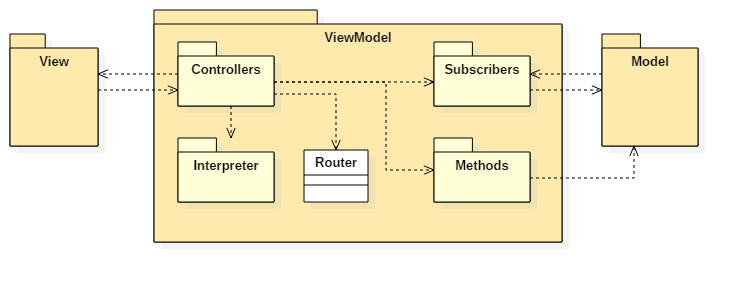
\includegraphics[scale=0.7]{../images/ViewModelPackage.png}
\end{center}
\end{figure}

\subsection{ViewModel::Subscribers}
\subsubsection{ViewModel::Subscribers::QuestionsSubscriber}
\begin{figure}[h!]
\begin{center}
	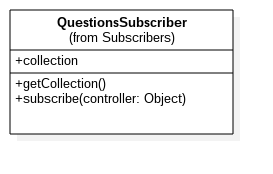
\includegraphics[scale=0.4]{../images/ViewModel/Subscribers/QuestionsSubscriber.png}
\end{center}
\end{figure}
\begin{itemize}
\item\textbf{Funzione del componente}: la classe è necessaria ad effettuare il \emph{subscribe} relativo alla collezione di domande del sistema;
	\item\textbf{Relazione d'uso con altre componenti}: \\
La classe utilizza:
	\begin{itemize}
		\item Model::Publishers::QuestionPublisher	
	\end{itemize}
\item\textbf{Attributi}:
	\begin{itemize}
		\item\code{- collection: String}: il nome della collezione sulla quale effettuare il subscribe.\\	
	\end{itemize}
\item\textbf{Metodi}:
	\begin{itemize}
		\item\code{+ getCollection(): String}: ritorna la collezione sulla quale può effettuare il subscribe.\\
		\textbf{Precondizioni}: viene richiesta la collezione di pertinenza della classe\\
		\textbf{Postcondizioni}: viene ritornato il nome della collezione\\
		\item\code{+ subscribe()}: metodo che effettua il subscribe del parametro controller alla collezione\\
		\textbf{Precondizioni}: viene richiesto di effettuare il subscribe del parametro controller alla collezione\\
		\textbf{Postcondizioni}: è stato effettuato il subscribe del controller alla collezione\\
		\textbf{Parametri}:
			\begin{itemize}
				\item\code{controller: Object}: il controller che necessita della collezione\\
			\end{itemize}
	\end{itemize}
\end{itemize}
\newpage

\subsubsection{ViewModel::Subscribers::QuizSubscriber}
\begin{figure}[h!]
\begin{center}
	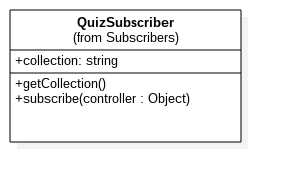
\includegraphics[scale=0.4]{../images/ViewModel/Subscribers/QuizSubscriber.png}
\end{center}
\end{figure}
\begin{itemize}
\item\textbf{Funzione del componente}: la classe è necessaria ad effettuare il \emph{subscribe} relativo alla collezione di quiz del sistema;
	\item\textbf{Relazione d'uso con altre componenti}:\\
La classe utilizza:
	\begin{itemize}
		\item Model::Publishers::QuizPublisher
	\end{itemize}
\item\textbf{Attributi}:
	\begin{itemize}
		\item\code{- collection: String}: il nome della collezione sulla quale effettuare il subscribe.\\	
	\end{itemize}
\item\textbf{Metodi}:
	\begin{itemize}
		\item\code{+ getCollection(): String}: ritorna la collezione sulla quale può effettuare il subscribe.\\
		\textbf{Precondizioni}: viene richiesta la collezione di pertinenza della classe\\
		\textbf{Postcondizioni}: viene ritornato il nome della collezione\\
		\item\code{+ subscribe()}: metodo che effettua il subscribe del parametro controller alla
		\textbf{Precondizioni}: viene richiesto di effettuare il subscribe del parametro controller alla collezione\\
		\textbf{Postcondizioni}: è stato effettuato il subscribe del controller alla collezione\\
		\textbf{Parametri}:
			\begin{itemize}
				\item\code{controller: Object}: il controller che necessita della collezione\\
			\end{itemize}
	\end{itemize}
\end{itemize}
\newpage

\subsection{ViewModel::Methods}
\subsubsection{ViewModel::Methods::QuestionMethods}
\begin{figure}[h!]
\begin{center}
	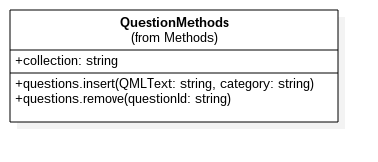
\includegraphics[scale=0.4]{../images/ViewModel/Methods/QuestionMethods.png}
\end{center}
\end{figure}
\begin{itemize}
\item\textbf{Funzione del componente}: permette al client di richiedere la modifica della collezione di domande del server;
	\item\textbf{Relazione d'uso con altre componenti}: \\
La classe utilizza:
	\begin{itemize}
		\item Model::Publishers::QuestionPublisher
		\item Model::Statistics::Statistics
	\end{itemize}
\item\textbf{Attributi}:
	\begin{itemize}
		\item\code{- collection: String}: la collezione sulla quale verranno implementati i methods\\
	\end{itemize}
\item\textbf{Metodi}:
	\begin{itemize}
		\item\code{+ questions.insert()}: metodo che inserisce una domanda nella collezione\\
		\textbf{Precondizioni}: viene richiesto di inserire una nuova domanda nella collezione\\
		\textbf{Postcondizioni}: la nuova domanda è stata salvata nel sistema\\
		\textbf{Parametri}:
			\begin{itemize}
				\item\code{QMLtext: string}: testo QML (corretto perchè viene prima parsato) corrispondente alla nuova domanda\\
				\item\code{category: string}: testo contente la categorie di appertenenza della domanda che si vuole inserire\\
			\end{itemize}
		\item\code{+ questions.remove()}: metodo che rimuove una domanda dalla collezione\\
		\textbf{Precondizioni}: viene richiesta l'eliminazione di una domanda dal sistema\\
		\textbf{Postcondizioni}: la domanda è stata eliminata dal sistema\\
		\textbf{Parametri}:
			\begin{itemize}
				\item\code{questionId: String}: identificativo univoco della domanda da rimuovere\\
			\end{itemize}
	\end{itemize}
\end{itemize}
\newpage

\subsubsection{ViewModel::Methods::QuizMethods}
\begin{figure}[h!]
\begin{center}
	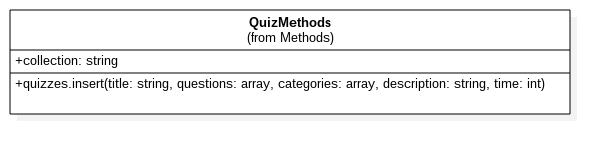
\includegraphics[scale=0.4]{../images/ViewModel/Methods/QuizMethods.png}
\end{center}
\end{figure}
\begin{itemize}
\item\textbf{Funzione del componente}: permette al client di richiedere la modifica della collezione di quiz del server;
	\item\textbf{Relazione d'uso con altre componenti}: \\
La classe utilizza:
	\begin{itemize}
		\item Model::Publishers::QuizPublisher
	\end{itemize}
\item\textbf{Attributi}:
	\begin{itemize}
		\item\code{- collection: String}: la collezione sulla quale verranno implementati i methods\\
	\end{itemize}
\item\textbf{Metodi}:
	\begin{itemize}
		\item\code{+ quizzes.insert()}: metodo che inserisce un quiz nella collezione\\
		\textbf{Precondizioni}: viene richiesto di inserire un nuovo quiz nella collezione\\
		\textbf{Postcondizioni}: il nuovo quiz è stato salvato nel sistema\\
		\textbf{Parametri}:
			\begin{itemize}
				\item\code{title: string}: contiene il titolo del nuovo questionario\\
				\item\code{questions: array}: elenca le domande presenti nel nuovo questionario\\
				\item\code{categories: array}: elenca le categorie di pertinenza del nuovo questionario\\
				\item\code{description: string}: contiene una breve descrizione testuale del questionario\\
				\item\code{time: int}: stabilisce il tempo massimo per la risoluzione del quiz\\
			\end{itemize}
		\item\code{+ quizzes.remove()}: metodo che rimuove un quiz dalla collezione\\
		\textbf{Precondizioni}: viene richiesta l'eliminazione di un quiz dal sistema\\
		\textbf{Postcondizioni}: il quiz è stato eliminato dal sistema\\
		\textbf{Parametri}:
			\begin{itemize}
				\item\code{quizId: String}: identificativo univoco della domanda da rimuovere\\
			\end{itemize}
	\end{itemize}
\end{itemize}
\newpage

\subsubsection{ViewModel::Methods::UserMethods}
\begin{figure}[h!]
\begin{center}
	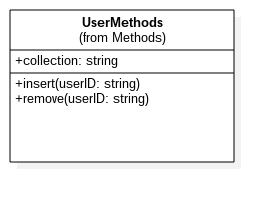
\includegraphics[scale=0.4]{../images/ViewModel/Methods/UserMethods.png}
\end{center}
\end{figure}
\begin{itemize}
\item\textbf{Funzione del componente}: permette al client di richiedere la modifica della collezione di utenti del server;
\item\textbf{Attributi}:
	\begin{itemize}
		\item\code{- collection: String}: la collezione sulla quale verranno implementati i methods\\
	\end{itemize}
\item\textbf{Metodi}:
	\begin{itemize}
		\item\code{+ insert()}: metodo che inserisce un utente nella collezione\\
		\textbf{Precondizioni}: viene richiesto di inserire un nuovo utente nella collezione\\
		\textbf{Postcondizioni}: il nuovo utente è stato salvato nel sistema\\
		\textbf{Parametri}:
			\begin{itemize}
				\item\code{userId: String}: identificativo univoco dell'utente da aggiungere\\
			\end{itemize}
		\item\code{+ remove()}: metodo che rimuove un utente dalla collezione\\
		\textbf{Precondizioni}: viene richiesta l'eliminazione di un utente dal sistema\\
		\textbf{Postcondizioni}: l'utente è stato eliminato dal sistema\\
		\textbf{Parametri}:
			\begin{itemize}
				\item\code{userId: String}: identificativo univoco dell'utente da rimuovere\\
			\end{itemize}
	\end{itemize}
\end{itemize}
\newpage

\subsection{ViewModel::Interpreter}
\subsubsection{ViewModel::Interpreter::Interpreter}
\begin{figure}[h!]
\begin{center}
	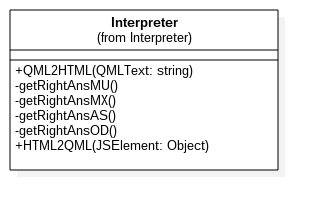
\includegraphics[scale=0.4]{../images/ViewModel/Interpreter/Interpreter.png}
\end{center}
\end{figure}
\begin{itemize}
\item\textbf{Funzione del componente}: interfaccia di base del tipo Interpreter.
	\item\textbf{Relazione d'uso con altre componenti}: viene concretizzata in ViewModel::Interpreter::QMLInterpreter.\\

\item\textbf{Attributi}: nessuno
\item\textbf{Metodi}:
	\begin{itemize}
		\item\code{+ translate(): String}: metodo astratto per la traduzione di un testo\\
		\textbf{Precondizioni}: viene richiesta la traduzione di un testo\\
		\textbf{Postcondizioni}: il testo è stato tradotto in un altro linguaggio\\
		\textbf{Parametri}:
			\begin{itemize}
				\item\code{data: String}: l'input testuale che deve essere tradotto \\
			\end{itemize}
	\end{itemize}
\end{itemize}
\newpage

\subsection{ViewModel::Router}
\subsubsection{ViewModel::Router::Router}
\begin{figure}[h!]
\begin{center}
	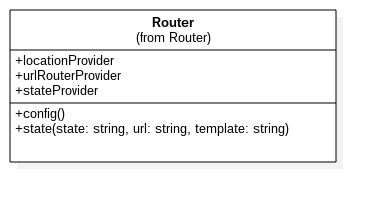
\includegraphics[scale=0.4]{../images/ViewModel/Router/Router.png}
\end{center}
\end{figure}
\begin{itemize}
\item\textbf{Funzione del componente}: implementa il routing dinamico dell'applicazione. Permette di dividere la parte statica dell'applicazione dalla parte che viene elaborata dinamicamente;
\item\textbf{Attributi}:
	\begin{itemize}
		\item\code{\$locationProvider: \$locationProvider}: provider AngularJs per rendere gli Url più leggibili\\
		\item\code{\$urlRouterProvider: \$urlRouterProvider}: modulo del package ui-router per definire il routing di default dell'applicazione\\
		\item\code{\$stateProvider: \$stateProvider}: modulo del package ui-router per mappare gli Url al caricamento dinamico dei template dell'applicazione. Tale associazione è definita come uno 'state'\\
	\end{itemize}
\item\textbf{Metodi}:
	\begin{itemize}
		\item\code{config()}: si occupa di gestire le varie chiamate del metodo state() all'inizializzazione dell'applicazione\\
		\textbf{Precondizioni}: l'applicazione Quizzipedia viene avviata\\
		\textbf{Postcondizioni}: tutti i template sono disponibili al caricamento\\
		\item\code{state()}: metodo per collegare un Url dell'applicazione al rispettivo template da caricare\\
		\textbf{Precondizioni}: viene richiesta l'associazione di un Url al caricamento di un template\\
		\textbf{Postcondizioni}: un Url univoco è stato associato al caricamento dinamico di uno specifico template\\
		\textbf{Parametri}:
			\begin{itemize}
				\item\code{state: String}: il nome dello stato rappresentato dall'associazione Url-Template\\
				\item\code{url: String}: l'Url sul quale effettuare il matching\\
				\item\code{template: String}: il template da caricare una volta trovato il match\\
			\end{itemize}
	\end{itemize}
\end{itemize}
\newpage

\subsection{ViewModel::Controller}
\subsubsection{ViewModel::Controller::QuestionList}
\begin{figure}[h!]
\begin{center}
	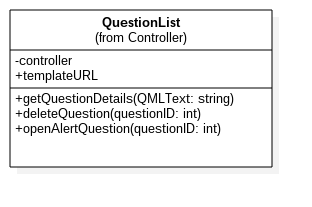
\includegraphics[scale=0.4]{../images/ViewModel/Controller/QuestionList.png}
\end{center}
\end{figure}
\begin{itemize}
\item\textbf{Funzione del componente:} visualizza una lista di domande
				\item\textbf{Relazioni d'uso con altre componenti:} \\
La classe si relaziona con:
	\begin{itemize}
		\item View::Templates::Question
		\item View::Templates::QuestionList
		\item Model::Publishers::QuestionPublishers
		\item ViewModel::Interpreter::Interpreter	
	\end{itemize}
\item\textbf{Funzionalità}:
\begin{itemize}
		\item\code{+ getQuestionDetails(QMLtext)}: restituisce i dettagli sulla domanda corrente se essa è valida;\\
		\item\code{+ deleteQuestion(questionID)}: richiede la rimozione dal database di una domanda;\\
		\item\code{+ openAlertQuestion(questionID)}: fornisce un messaggio pop-up di conferma all'utente;\\
	\end{itemize}
	\item\textbf{Attributi:}
	\begin{itemize}
	\item\code{+ controller: String}: variabile contenente il nome del controller del template;\\
 
 	\item\code{+ templateUrl: String}: stringa contenente il percorso del file HTML che contiene il template\\
	\end{itemize}
\end{itemize}
\newpage

\subsubsection{ViewModel::Controller::Question}
\begin{figure}[h!]
\begin{center}
	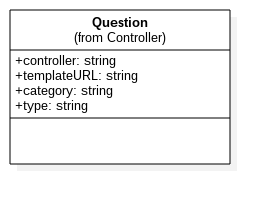
\includegraphics[scale=0.4]{../images/ViewModel/Controller/Question.png}
\end{center}
\end{figure}
\begin{itemize}
\item\textbf{Funzione del componente:} permette la visualizzazione di una singola domanda
				\item\textbf{Relazioni d'uso con altre componenti:} 
La classe è in relazione con:
\begin{itemize}
		\item View::Templates::Question
		\item View::Templates::QuestionList
	\end{itemize}
\item\textbf{Attributi}:
	\begin{itemize}
		\item\code{+ controller: String}: variabile contenente il nome del controller del template;\\

		\item\code{+ templateUrl: String}: stringa contenente il percorso del file HTML che contiene il template\\
		\item\code{+ category: String}: stringa contenente la categoria della domanda
 		\item\code{+ type: String}: stringa contenente il tipo della domanda
	\end{itemize}
\end{itemize}
\newpage

\subsubsection{ViewModel::Controller::QuizList}
\begin{figure}[h!]
\begin{center}
	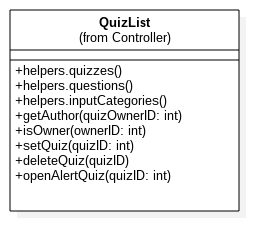
\includegraphics[scale=0.4]{../images/ViewModel/Controller/QuizList.png}
\end{center}
\end{figure}
\begin{itemize}
\item\textbf{Funzione del componente:} permette visualizzazione e interazione di una lista di questionari
				\item\textbf{Relazioni d'uso con altre componenti:}\\
La classe utilizza:
	\begin{itemize}
		\item View::Templates::Quiz
		\item Model::Publishers::QuizPublishers
		\item Model::Publishers::QuestionPublishers
		\item Model::Parser::Parser
	\end{itemize}
\item\textbf{Funzionalità}:
	\begin{itemize}
		\item\code{+ helpers.quizzes()}: restituisce i questionari della categoria ricercata;\\
		\item\code{+ helpers.questions()}: restituisce le domande contenute nel questionario selezionato;\\
		\item\code{+ helpers.inputCategories()}: recupera tutte le categorie dei quiz per popolare la select senza inserire duplicati;\\
		\item\code{+ getAuthor(quizOwnerID)}: restituisce l'autore del quiz selezionato\\
		\item\code{+ isOwner(ownerID)}: restituisce un esito positivo se il creatore del quiz è l'utente attualmente loggato\\
		\item\code{+ setQuiz(qID}: richiede il questionario scelto dall'utente per il caricamento dal database\\
		\item\code{+ deleteQuiz(quiz)}: permette l'eliminazione del quiz scelto\\
		\item\code{+ openAlertQuiz(quizID)}: fornisce un messaggio pop-up di conferma all'utente;\\
	\end{itemize}
\end{itemize}
\newpage

\subsubsection{ViewModel::Controller::Quiz}
\begin{figure}[h!]
\begin{center}
	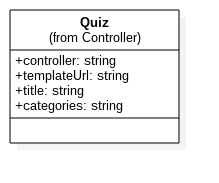
\includegraphics[scale=0.4]{../images/ViewModel/Controller/Quiz.png}
\end{center}
\end{figure}
\begin{itemize}
\item\textbf{Funzione del componente:} visualizza un quiz inserito in una lista
				\item\textbf{Relazioni d'uso con altre componenti:}\\
 La classe è utilizzata da:
 	\begin{itemize}
 		\item View::Templates::QuizList
 		\item View::Templates::Quiz
 		\item View::Templates::QuestionList
 	\end{itemize}
 \item\textbf{Attributi}:
 	\begin{itemize}
 		\item\code{+ controller: String}: variabile contenente il nome del controller del template;\\
		
		\item\code{+ templateUrl: String}: stringa contenente il percorso del file HTML che contiene il template\\
		\item\code{title: String}: stringa contenente il titolo del quiz
		\item\code{categories: String}: stringa contenente le categorie del quiz
 	\end{itemize}
 \end{itemize}
\newpage

 \subsubsection{ViewModel::Controller::QuestionForm}
 \begin{figure}[h!]
\begin{center}
	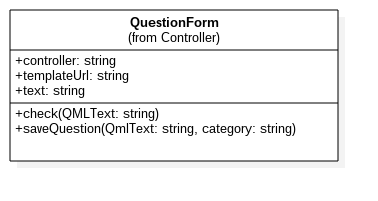
\includegraphics[scale=0.4]{../images/ViewModel/Controller/QuestionForm.png}
\end{center}
\end{figure}
 \begin{itemize}
 \item\textbf{Funzione del componente:} visualizza il form utilizzabile sia per la creazione che per la modifica di una domanda
 \item\textbf{Attributi}:
 	\begin{itemize}
 		\item\code{+ controller: String}: variabile contenente il nome del controller del template;\\
		
		\item\code{+ templateUrl: String}: stringa contenente il percorso del file HTML che contiene il template\\
		\item\code{+ category: String}: stringa contenente la categoria della domanda
		\item\code{+ text: String}: stringa contenente il testo della domanda
 	\end{itemize}
 	\item\textbf{Metodi}:
 	\begin{itemize}
 		\item\code{+ check(QMLtext)}: si occupa della verifica della correttezza del testo QML inserito dall'utente;\\
 		\item\code{+ saveQuestion(QMLtext, category)}: salva le modifiche effettuate su una domanda;\\
 	\end{itemize}
 \end{itemize}
\newpage
 
 \subsubsection{ViewModel::Controller::QuizCreationForm}
 \begin{figure}[h!]
\begin{center}
	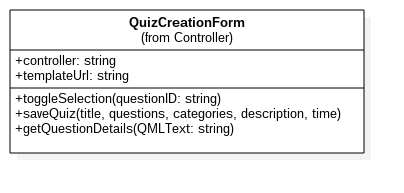
\includegraphics[scale=0.4]{../images/ViewModel/Controller/QuizCreationForm.png}
\end{center}
\end{figure}
 \begin{itemize}
 \item\textbf{Funzione del componente:} visualizza il form di creazione di un questionario
 \item\textbf{Relazione d'uso con altri componenti}:
 \begin{itemize}
 	\item View::Pages::QuizCreationPage
 	\item Model::Publishers::QuestionPublishers
 \end{itemize}
 \item\textbf{Attributi}:
 	\begin{itemize}
 		\item\code{+ controller: String}: variabile contenente il nome del controller del template;\\
		
		\item\code{+ templateUrl: String}: stringa contenente il percorso del file HTML che contiene il template\\
 	\end{itemize}
 	\item\textbf{Metodi};
 	\begin{itemize}
 		\item\code{+ toggleSelection(questionID)}: si occupa di gestire la selezione della domanda da inserire nel questionario attualmente in fase di creazione;\\
 		\item\code{+ savequiz(title,questions,categories,description,time)}:
 		gestisce il salvataggio del questionario;\\
 		\item\code{+ getQuestionDetails(QMLtext)}: fornisce informazioni su una specifica domanda candidata all'inserimento nel questionario;\\
 	\end{itemize}
 \end{itemize}
\newpage
 
 \subsubsection{ViewModel::Controller::QuestionCompilation}
 \begin{figure}[h!]
\begin{center}
	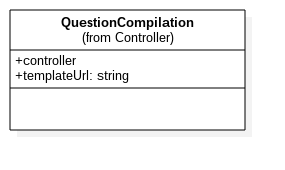
\includegraphics[scale=0.4]{../images/ViewModel/Controller/QuestionCompilation.png}
\end{center}
\end{figure}
 \begin{itemize}
 \item\textbf{Funzione del componente:} visualizza una domanda e ne permette la compilazione
 \item\textbf{Relazioni con altre componenti}\\
 La classe utilizza:
 	\begin{itemize}
 		\item View::Templates::Question
 		\item View::Templates::QuizResults
 	\end{itemize}
 \item\textbf{Attributi}:
 	\begin{itemize}
 		\item\code{+ controller: String}: variabile contenente il nome del controller del template;\\
		
		\item\code{+ templateUrl: String}: stringa contenente il percorso del file HTML che contiene il template\\
 	\end{itemize}
 \end{itemize}
\newpage
 
 \subsubsection{ViewModel::Controller::QuizResults}
 \begin{figure}[h!]
\begin{center}
	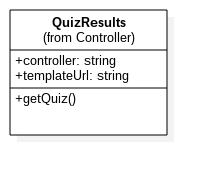
\includegraphics[scale=0.4]{../images/ViewModel/Controller/QuizResults.png}
\end{center}
\end{figure}
 \begin{itemize}
 \item\textbf{Funzione del componente:} visualizza i risultati ottenuti in seguito alla compilazione di un quiz
 \item\textbf{Relazioni con altre componenti}\\
 La classe utilizza:
 	\begin{itemize}
 		\item View::Templates::QuestionCompilation
 		\item View::Templates::QuizResults
 	\end{itemize}
 \item\textbf{Attributi}:
 	\begin{itemize}
 		\item\code{+ controller: String}: variabile contenente il nome del controller del template;\\
		\item\code{+ templateUrl: String}: stringa contenente il percorso del file HTML che contiene il template\\
 	\end{itemize}
 	\item\textbf{Metodi}:
 	\begin{itemize}
 		\item\code{+ getQuiz()}: si occupa di fornire il punteggio finale
 	\end{itemize}
 \end{itemize}
\newpage
 
 \subsubsection{ViewModel::Controller::SearchForm}
 \begin{figure}[h!]
\begin{center}
	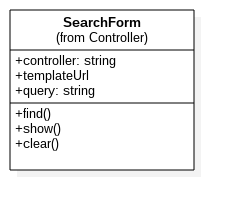
\includegraphics[scale=0.4]{../images/ViewModel/Controller/SearchForm.png}
\end{center}
\end{figure}
 \begin{itemize}
 \item\textbf{Funzione del componente:} visualizza una form per l’inserimento dei dati desiderati e l’avvio della ricerca
 \item\textbf{Attributi}:
 	\begin{itemize}
 		\item\code{+ controller: String}: variabile contenente il nome del controller del template;\\
		
		\item\code{+ templateUrl: String}: stringa contenente il percorso del file HTML che contiene il template\\
		\item\code{+ query: String}: stringa contenente la query da sottomettere al sistema\\
 	\end{itemize}
 	\item\textbf{Funzionalità}:
 	\begin{itemize}
 		\item\code{+ find():} esegue l'effettiva attività di ricerca nel sistema\\
		\item\code{+ show():} fornisce la rappresentazione grafica dei risultati\\
		\item\code{+ clear():} metodo di servizio per la pulizia dell'interfaccia\\
 	\end{itemize}
 \end{itemize}
\newpage
 
 \subsubsection{ViewModel::Controller::NavBar}
 \begin{figure}[h!]
\begin{center}
	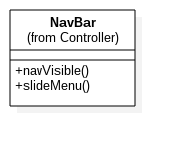
\includegraphics[scale=0.4]{../images/ViewModel/Controller/NavBar.png}
\end{center}
\end{figure}
 \begin{itemize}
 \item\textbf{Funzione del componente:} Fornisce un menù laterale che facilita l'interazione dell'utente con l'applicazione
 \item\textbf{Relazione con altri componenti:}
 \begin{itemize}
 	\item View::Templates::navbar
 \end{itemize}
 \item\textbf{Funzionalità}:
 	\begin{itemize}
 		\item\code{+ navVisible():} imposta la larghezza del menù laterale\\
		\item\code{+ slideMenu():} gestisce effetti grafici responsive\\
 	\end{itemize}
 \end{itemize}
\newpage
 
 \subsubsection{ViewModel::Controller::TopBar}
 \begin{figure}[h!]
\begin{center}
	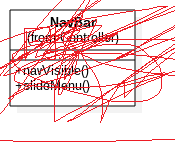
\includegraphics[scale=0.4]{../images/ViewModel/Controller/TopBar.png}
\end{center}
\end{figure}
 \begin{itemize}
 \item\textbf{Funzione del componente:} Fornisce il menù orizzontale con cui l'utente può interfacciarsi con il sistema
 \item\textbf{Relazione con altri componenti:}
 \begin{itemize}
 	\item View::Templates::topbar
 \end{itemize}
 \end{itemize}
\newpage
 
  \subsubsection{ViewModel::Controller::UserProfile}
  \begin{figure}[h!]
\begin{center}
	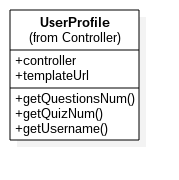
\includegraphics[scale=0.4]{../images/ViewModel/Controller/UserProfile.png}
\end{center}
\end{figure}
 \begin{itemize}
 \item\textbf{Funzione del componente:} permette la visualizzazione e l'interazione dell'utente con il proprio profilo e le funzionalità da esso offerto\\
 \item\textbf{Relazione con altri componenti:}
 \begin{itemize}
 	\item View::Templates::UserProfile
 	\item ViewModel::Controller::QuestionList
 	\item ViewModel::Controller::QuizList
 	\item Model::Publishers::QuestionPublishers
 	\item Model::Publishers::QuizPublishers
 \end{itemize}
 \item\textbf{Attributi:}
 \begin{itemize}
 	\item\code{+ controller: String}: variabile contenente il nome del controller del template;\\
		\item\code{+ templateUrl: String}: stringa contenente il percorso del file HTML che contiene il template\\
 \end{itemize}
 \item\textbf{Metodi:}
 	\begin{itemize}
 		\item\code{+ getQuestionsNum():} ritorna la quantità di domande create dallo stesso utente;\\
		\item\code{+ getQuizNum():} ritorna la quantità di questionari creati dallo stesso utente;\\
		\item\code{+ getUsername():} ritorna il nome dell'utente loggato;\\
 	\end{itemize}
 \end{itemize}
\newpage
 
 \subsubsection{ViewModel::Controller::QuizHome}
 \begin{figure}[h!]
\begin{center}
	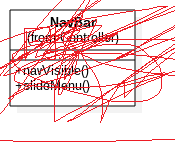
\includegraphics[scale=0.4]{../images/ViewModel/Controller/QuizHome.png}
\end{center}
\end{figure}
 \begin{itemize}
 \item\textbf{Funzione del componente:} 
 \item\textbf{Relazione con altri componenti:}
 \begin{itemize}
	\item V
 \end{itemize}
 \item\textbf{Attributi:}
 \begin{itemize}
	\item a
 \end{itemize}
 \item\textbf{Metodi:}
 	\begin{itemize}
\item V
 	\end{itemize}
 \end{itemize}
\newpage

 \subsubsection{ViewModel::Controller::QuizStatistics}
 \begin{figure}[h!]
\begin{center}
	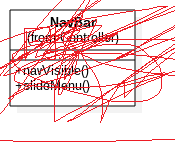
\includegraphics[scale=0.4]{../images/ViewModel/Controller/QuizStatistics.png}
\end{center}
\end{figure}
  \begin{itemize}
 \item\textbf{Funzione del componente:} 
 \item\textbf{Relazione con altri componenti:}
 \begin{itemize}
		\item V
 \end{itemize}
 \item\textbf{Attributi:}
 \begin{itemize}
\item a
 \end{itemize}
 \item\textbf{Metodi:}
 	\begin{itemize}
\item wddwdad
 	\end{itemize}
 \end{itemize}
\newpage

 \subsubsection{ViewModel::Controller::QuizCompilation}
 \begin{figure}[h!]
\begin{center}
	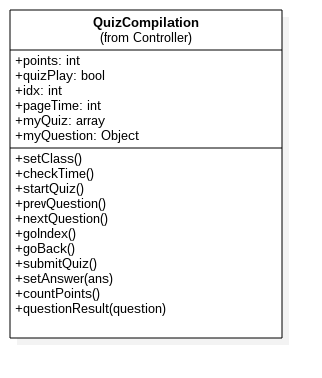
\includegraphics[scale=0.4]{../images/ViewModel/Controller/QuizCompilation.png}
\end{center}
\end{figure}
  \begin{itemize}
 \item\textbf{Funzione del componente:} 
 \item\textbf{Relazione con altri componenti:}
 \begin{itemize}
\item afewf
 \end{itemize}
 \item\textbf{Attributi:}
 \begin{itemize}
		\item a
 \end{itemize}
 \item\textbf{Metodi:}
 	\begin{itemize}
\item faf
 	\end{itemize}
 \end{itemize}
